\documentclass[12pt,a4paper]{article}
\usepackage[margin=2.5cm]{geometry}
\usepackage{amsmath,amssymb,graphicx,setspace,palatino, subcaption}
\usepackage[hidelinks]{hyperref}

\captionsetup[figure]{labelfont=bf,textfont={small,normalfont}}
%\captionsetup[subfigure]{labelsep=quad, labelfont={bf,small}, textfont=small, singlelinecheck=off, justification=raggedright, position=top}
%\renewcommand{\thesubfigure}{\Alph{subfigure}}

\renewcommand*{\thefootnote}{\fnsymbol{footnote}}
\setcounter{footnote}{1}

\begin{document}

\onehalfspacing

\section{Introduction}

\section{Results}

In this work, we developed mathematical models to estimate the rates and probabilities of \textit{de novo} gene emergence, as well as gene loss. A \textit{de novo} gene emerges from a non-genic DNA, when the latter mutates to gain sequence features necessary for transcription and translation. Both transcription and translation are complex processes involving many biomolecular complexes that work in concert. Here, we focus on the minimal requirements for these processes to occur. Specifically for transcription, we require a gene to have one of the two core promoter motifs, the TATA-box or the Initiator element (Inr), and a polyadenylation (poly-A) signal sequence. For translation, we only require the gene to have an open reading frame (ORF). Using simple probability models, we calculate the likelihood of finding these features in a DNA sequence by random chance, and the rate at which these features are gained and lost via mutagenesis. Using a similar approach, we estimate some fundamental biochemical properties of proteins that arise from random DNA sequences. Our models thus define a null hypothesis under which DNA sequences evolve neutrally through mutation pressure alone. A significant deviation from this null hypothesis may be interpreted as evidence in support of natural selection. 

\subsection{How many times can a gene be lost?}

If a gene is found in one species but not in sister taxa, then the most common assumption is that this gene emerged only in one specific species. We asked what is the chance that the gene was present in a common ancestor, but was lost in all lineages except one. To this end we calculated the probability of gene emergence and gene loss (Materials and Methods). Specifically, the probability of gene gain can be defined as the sum of three probabilities. First is the probability that an ORF already exists, and a mutation causes transcription to emerge ($P_\textit{RNA-gain}$) but doesn't disrupt the ORF ($P_\textit{ORF-stay}$). Second is the probability that the DNA is transcribed, and an ORF emerges due to mutations ($P_\textit{ORF-gain}$) while transcription stays intact ($P_\textit{RNA-stay}$). Third is the probability that neither of the two features already exist and both emerge at the same time due to mutations (this probability is very small, and negligible). The following equation describes the probability of gene gain\footnote{\autoref{genegaineq} describes total gene gain probability. Gene gain probability conditioned on the gene being absent would be $P_\textit{gene-gain}/(1-P_\textit{ORF} - P_\textit{RNA})$. Using this value does not change the results significantly.}:

\begin{equation}
P_\textit{gene-gain} = P_\textit{ORF-stay}\times P_\textit{RNA-gain} + P_\textit{RNA-stay}\times P_\textit{ORF-gain} + P_\textit{RNA-gain}\times P_\textit{ORF-gain}
\label{genegaineq}
\end{equation}

Likewise, the probability of gene loss, given the gene (transcription and ORF) is already present, is the sum of the probabilities that transcription ($P_\textit{RNA-loss}$) or the ORF is lost due to mutations ($P_\textit{ORF-loss}$) due to mutations. Specifically:

\begin{equation}
P_\textit{gene-loss} = P_\textit{RNA-loss} + P_\textit{ORF-loss}
\label{genelosseq}
\end{equation}

The probability that a gene is lost $n$ times independently, is $(P_\textit{gene-loss})^{n}$. To find out how many independent gene loss events are as likely as a single gene gain event, we calculate the ratio of logarithms of gene gain and gene loss: $\log(P_\textit{gene-gain})/\log(P_\textit{gene-loss})$. For example, the ratio value of 2 would indicate that two independent gene loss events are as likely as a single gene gain event. We calculated this ratio for genes with different ORF lengths, because ORF gain and loss probabilities depend on the length of the ORF. We found that for all ORF lengths, the gene can be lost at least two times independently, in the time required to gain it (\autoref{gainlossprob}). 

\begin{figure}[!t]
\centering
\includegraphics[scale=0.6]{Figures/geneGainLoss.pdf}
\caption{Genes are more likely to be independently lost twice, than being born once. The vertical axis shows the number of independent gene loss events than can happen relative to one gene gain event i.e. $\log(P_\textit{gene-gain})/\log(P_\textit{gene-loss})$. The horizontal axis shows the number of codons in the ORF.}
\label{gainlossprob}

\vspace{1ex}
\hrule
\end{figure}

We performed the same analysis to just the ORF (and not the whole genes). That is, we calculated the ratio of logarithms of ORF gain and ORF loss. We found that for ORFs longer than 143 codons, the likelihood of two independent ORF loss events is more than or equal to a single ORF gain event. 

Overall, our analysis suggests that \textit{de novo} gene expressed in only one species may not necessarily mean that it emerged for the first time in this species. 

\subsection{Does \textit{de novo} gene emergence have a preferred trajectory?}

\begin{figure}[!b]
\hrule
\vspace{1ex}
\centering
%\begin{subfigure}{0.48\textwidth}
%\centering
%\caption{One-step}
\includegraphics[scale=0.6]{Figures/first_ORF_RNA.pdf}
%\end{subfigure}\hfill%
%\begin{subfigure}{0.48\textwidth}
%\centering
%\caption{Two-step}
%\includegraphics[scale=0.6]{Figures/first_ORF_RNA2.pdf}
%\end{subfigure}
\caption{\textit{De novo} genes with shorter ORFs ($<$ 42 codons) preferentially emerge from existing ORFs (ORF-first) whereas \textit{de novo} genes with longer ORFs preferentially emerge from existing RNAs (RNA-first). The horizontal axis denotes the number of codons in the ORF. The vertical axis shows the log transformed ratio of single-step probabilities of ORF-first and RNA-first trajectories of \textit{de novo} emergence (Equations \ref{orffirsteq1} \& \ref{rnafirsteq1}). A positive value suggests a ORF-first trajectory and a negative value supports RNA-first trajectory. Similar analysis with two-step probabilities shows a smaller difference between the likelihood of the two trajectories (Equations \ref{orffirsteq2} \& \ref{rnafirsteq2}).}
\label{whoisfirst}
\end{figure}

For a \textit{de novo} gene to emerge from a non-genic DNA sequence, both transcription and ORF need to emerge. That is, probability of gene emergence is equal to the product of probabilities of transcription gain and ORF gain. Thus it may appear that the order of the occurrence of these two events does not matter. Gene gain is much more likely when one of the two features already exist (\autoref{genegaineq}) and hence there are two possible trajectories -- ORF emerges first (ORF-first) or transcription emerges first (RNA-first). To test the hypothesis that the order of feature gain events influences \textit{de novo} emergence, we first asked how much more likely it is to lose transcription before gaining an ORF. Specifically, we calculated the fold difference between the probability values of transcription loss and ORF gain. We found that transcription loss is $10^3$ to $10^{10}$ times higher than ORF gain, depending on the ORF length. This suggests that a mutation has a higher chance of disrupting an existing untranscribed ORF than cause a gain of transcription features. Next, we calculated the fold difference between transcription gain and ORF loss probability values, and found that ORF loss is $10^4$ to $10^5$ times more probable than transcription gain, suggesting that in a transcribed DNA region, a new mutation will more likely disrupt the transcription features than cause a gain of ORF. More generally features are more easily lost due to mutations than they are gained. However, this effect of mutations is not uniform for the two evolutionary trajectories and for different length of ORFs. For example, gain of an 40 codon long ORF in a transcribed region of DNA is $9.2\times10^3$ less likely than the transcription being lost. However, if the ORF already exists, then it is $2.7\times10^4$ times more likely to be lost before transcription emerges. This suggests that the two trajectories of \textit{de novo} emergence have different dynamics.

To better understand whether \textit{de novo} gene emergence has a preferred trajectory, we calculated two probabilities. First is the probability that ORF exists and a mutation causes gain of transcription but no disruption of the ORF. This probability denotes the trajectory where ORF emerges first. 

\begin{equation}
P_\textit{ORF-first} = P_\textit{ORF-stay}\times P_\textit{RNA-gain}
\label{orffirsteq1}
\end{equation}

The second probability that denotes the trajectory where transcription emerges first, is the probability that DNA is already transcribed and a mutation causes gain of ORF but does not abolish transcription. 

\begin{equation}
P_\textit{RNA-first} = P_\textit{RNA-stay}\times P_\textit{ORF-gain}
\label{rnafirsteq1}
\end{equation}

We calculated the log-transformed ratio of $P_\textit{ORF-first}$ and $P_\textit{RNA-first}$, such that a positive value of the ratio would mean that transcription gain for an untranscribed ORF (ORF-first) is more likely than ORF gain in an already transcribed DNA (RNA-first). In other words, ORF-first hypothesis is more feasible. Likewise, a negative value of the ratio would suggest that RNA-first hypothesis is more feasible. With the specific parameter values we used, it turns out that \textit{de novo} genes with up to 42 codons in their coding region, preferentially emerge ORF-first. \textit{De novo} genes with longer coding region, emerge transcription first (\autoref{whoisfirst}).

A more stringent definition of ORF-first hypothesis would describe a two-step process. In the first step, an ORF emerges in an untranscribed region of DNA, but transcription does not emerge. In the second step transcription emerges, while ORF stays intact (\autoref{orffirsteq2})\footnote{$P_\textit{ORF-gain}$ describes the total probability of ORF emerging from a DNA region that does not have already have an ORF. Conditional probability of ORF gain would be $P_\textit{ORF-gain}/(1-P_\textit{ORF})$. Conditional probability of transcription gain can be described similarly.} . Likewise, RNA-first hypothesis can be defined by a two-step probability. In the first step transcription emerges in a non-genic DNA (that does not have an ORF), and in the second step an ORF emerges, while transcription remains intact (\autoref{rnafirsteq2}).

With this stringent definition, the difference between the probabilities of the two trajectories becomes very small ($< 3\times10^{-5}$). However, we still find that \textit{de novo} genes with shorter ORFs ($<$ 34 codons) have a slightly higher chance of emerging ORF first.

Overall, our analysis suggests that \textit{de novo} genes with long ORFs are more likely arise from DNA regions that are already transcribed (for example, non-coding RNAs). 

\begin{align}
P_\textit{ORF-first}' & = \underbrace{P_\textit{ORF-gain} \times (1-P_\textit{RNA} -P_\textit{RNA-gain})}_\textit{first step} \times \underbrace{P_\textit{ORF-stay}\times P_\textit{RNA-gain}/(1-P_\textit{RNA})}_\textit{second step} \label{orffirsteq2}\\[1em]
P_\textit{RNA-first}' & = \underbrace{P_\textit{RNA-gain} \times (1-P_\textit{ORF} -P_\textit{ORF-gain})}_\textit{first step} \times \underbrace{P_\textit{RNA-stay}\times P_\textit{ORF-gain}/(1-P_\textit{ORF})}_\textit{second step}\label{rnafirsteq2}
\end{align}

\subsection{Would extensive transcription loss suggest negative selection of toxic proteins?}


\textit{De novo} genes that do not provide any fitness benefit to an organism are not fixed in populations via natural selection. These genes can be lost due to mutation pressure. Some newborn \textit{de novo} genes can also encode toxic proteins, that may aggregate or interfere with physiology in some other way. These genes would thus be eliminated from the population genomes via negative selection. We remind the reader that an ORF is lost if the start codon is mutated, the stop codon is mutated to an amino acid encoding codon (non-stop mutation), or if an amino acid encoding codon is mutated to a stop codon (premature stop/non-sense mutation). It is likely that a non-stop mutation or a non-sense mutation, can still result in translation of a protein (extended or truncated, respectively). Furthermore, non-stop mutations can also lead to cellular toxicity. Thus ORF loss does not ensure elimination of toxic proteins, which in turn suggests that transcription loss may be the better way to inactivate the associated genes.

To understand which is the most probable mechanism of gene loss, we compared the probabilities of ORF loss ($P_\textit{ORF-loss}$) and transcription loss ($P_\textit{RNA-loss}$). We found that ORF loss is more probable than transcription loss, for all ORF longer than 33 codons (\autoref{lossprob}).

We reframed our question to make it more relatable to commonly observed findings from genomics experiments. For example, a hypothetical experiment involves DNA sequencing of a genomic locus in different related species. This experiment shows that transcription features are present in only one species, whereas the ORF is present in all species. Two evolutionary events could describe this observation. First possibility is that a \textit{de novo} gene existed in an ancestor and transcription was lost in multiple species. For any one species, the probability of this evolutionary trajectory is: $P_\textit{ORF-stay}\times P_\textit{RNA} \times P_\textit{RNA-loss}$ \footnote{Note that $P_\textit{RNA-loss}$ is a conditional probability dependent on the presence of RNA.}

\begin{figure}[!t]
\centering
\includegraphics[scale=0.6]{Figures/pLoss.pdf}
\caption{ORF loss is more probable than transcription loss, for \textit{de novo} genes containing more than 33 codons. The horizontal axis denotes the number of codons in the ORF. The vertical axis shows the log transformed ratio of ORF loss and RNA loss probabilities, such that a positive value means ORF-loss is more probable than RNA loss, and \textit{vice versa}.}
\label{lossprob}

\vspace{1ex}
\hrule
\end{figure}

Alternatively, an ORF could have existed in all species and transcription was subsequently gained in one species. The probability that this event happens in any one species is: $P_\textit{ORF-stay}\times P_\textit{RNA-gain}$ (see \autoref{orffirsteq1}). 

The ratio of the probabilities of the two evolutionary trajectories would simply be: $P_\textit{RNA} \times P_\textit{RNA-loss}/P_\textit{RNA-gain}$. We found the value of this ratio to be 0.914, suggesting that transcription loss in a \textit{de novo} gene would be more probable than transcription gain for an untranscribed ORF. However, this difference is small and hence the real evolutionary mechanism behind the observation from our hypothetical sequencing experiment, would be difficult to infer. 

In sum, transcription loss cannot be reliably inferred as an evidence for negative selection of protein expression.

\subsection{Does mutation bias shape protein composition?}

In previous sections, we showed that mutation bias affects the rate of \textit{de novo} gene emergence and loss. We next turned our attention to whether this bias affects the composition (and thereby the chemistry) of \textit{de novo} proteins. To this end, we first asked if the expected frequency of different amino acids is uniform, and found that it is not uniform. Amino acids like leucine (L) and serine (S) have a higher expected frequency than other amino acids. On the other hand, amino acids like methionine (M) and tryptophan (W) are less probable (\autoref{aafreq}). This non-uniformity is to a great extent determined by number of degenerate codons for an amino acid. However, GC content also plays a role. For example, leucine, arginine and serine, all have six codons each. However, leucine is more probable than serine which in turn is more probable than arginine (\autoref{aafreq}). 

Previous studies have argued that hydrophobic amino acids are comprise 40\% of amino acids and can also easily arise due to mutation pressure. They based these conclusions on mutation rate bias estimated in bacteria. We asked if our model also makes similar predictions. To this end we calculated expected hydropathy in a protein sequence, based on expected frequency of different amino acids (\autoref{aafreq}) and their hydropathic index values (Kyte and Doolittle). We found that the expected hydropathy is $-0.08628$, which suggests that random protein sequences are not mostly hydrophobic. 

Next, we calculated the probability that any 

\begin{itemize}
\item expected hydropathy index = $-0.08628$
\item acid to basic rate is $1.3074\times$ higher than \textit{vice versa}. Conditional prob = $1.80543$
\item mutations do not preferentially create hydrophobic amino acid. Total prob ratio = 1.025, Conditional prob ratio = 0.971
\end{itemize}

\begin{figure}[!t]
\centering
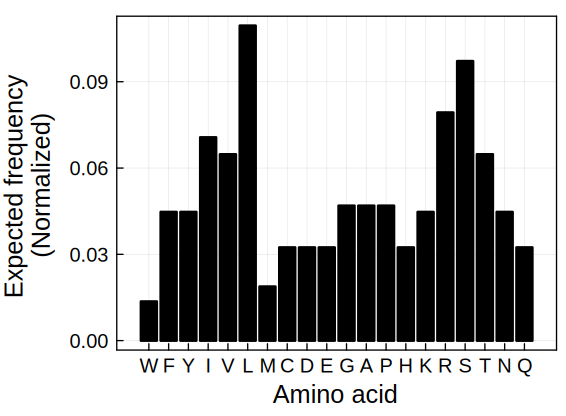
\includegraphics[scale=0.6]{Figures/pAAfreq.pdf}
\caption{ORF loss is more probable than transcription loss, for \textit{de novo} genes containing more than 33 codons. The horizontal axis denotes the number of codons in the ORF. The vertical axis shows the log transformed ratio of ORF loss and RNA loss probabilities, such that a positive value means ORF-loss is more probable than RNA loss, and \textit{vice versa}.}
\label{aafreq}

\vspace{1ex}
\hrule
\end{figure}

\section{Discussion} 




\end{document}
